\chapter{二项式定理}
相比于之前的乘法原理和加法原理,\textbf{二项式定理}(binomial theorem)比较简单,它主要研究形如$(a+b)^n$的展开问题。

\section{公式}
我们可以先从像引例\ref{lexpl:binomial-theorem}这样简单的问题开始思考起来。

\begin{lexample}\label{lexpl:binomial-theorem}
	$(a_1+b_1)(a_2+b_2)(a_3+b_3)$的展开式是什么?
\end{lexample}

\begin{proof}[解]
	很简单,将其展开共有8项,可得(这里省略一部分)\[a_1a_2a_3+a_1a_2b_3+a_1b_2a_3+\cdots+b_1b_2b_3\qedhere\]
\end{proof}

这样的展开是很有规律的,即在每一项中,1,2,3这3个下标都出现但只出现一次,不可能出现$a_1a_2b_2$的情况。

这虽然是个简单的代数问题,但当指数处再增大一些,就麻烦了.那我们何不变化思路,将其变成一个排列组合的问题?

以$(a+b)^3$为例,每一项都是3个数相乘,即我们要从3个括号中的每一个括号里各选一个数组成一项,共有$a^3,a^2b,ab^2,b^2$这4项,每项的系数则可以看作是从$n$个$a$(或$n$个$b$)中选$k$个有多少种选法。

所以,我们可以总结二项式$(a+b)^n$展开的通项公式\[T_{r+1}=C_n^ra^{n-r}b^r=C_n^ra^rb^{n-r}\]其中,$r$可以从0取到$n$. 这里的$C_n^r$叫作每一项的\textbf{二项式系数}(binomial coefficients)。

如果对通项公式中$a$和$b$的指数可以互换感到奇怪,可以回顾公式\eqref{equ:comb-1},这无非就是将展开式颠倒了罢了。

另外,我们也可以使用如图\ref{fig:pascals-triangle}的\textbf{杨辉三角形}或\textbf{帕斯卡三角形}(Pascal's triangle)来得到二项式系数。例如:第4行对应的二项式的指数是3,对应项的二项式系数是1,3,3,1。

\begin{figure}[htb]
	\centering
	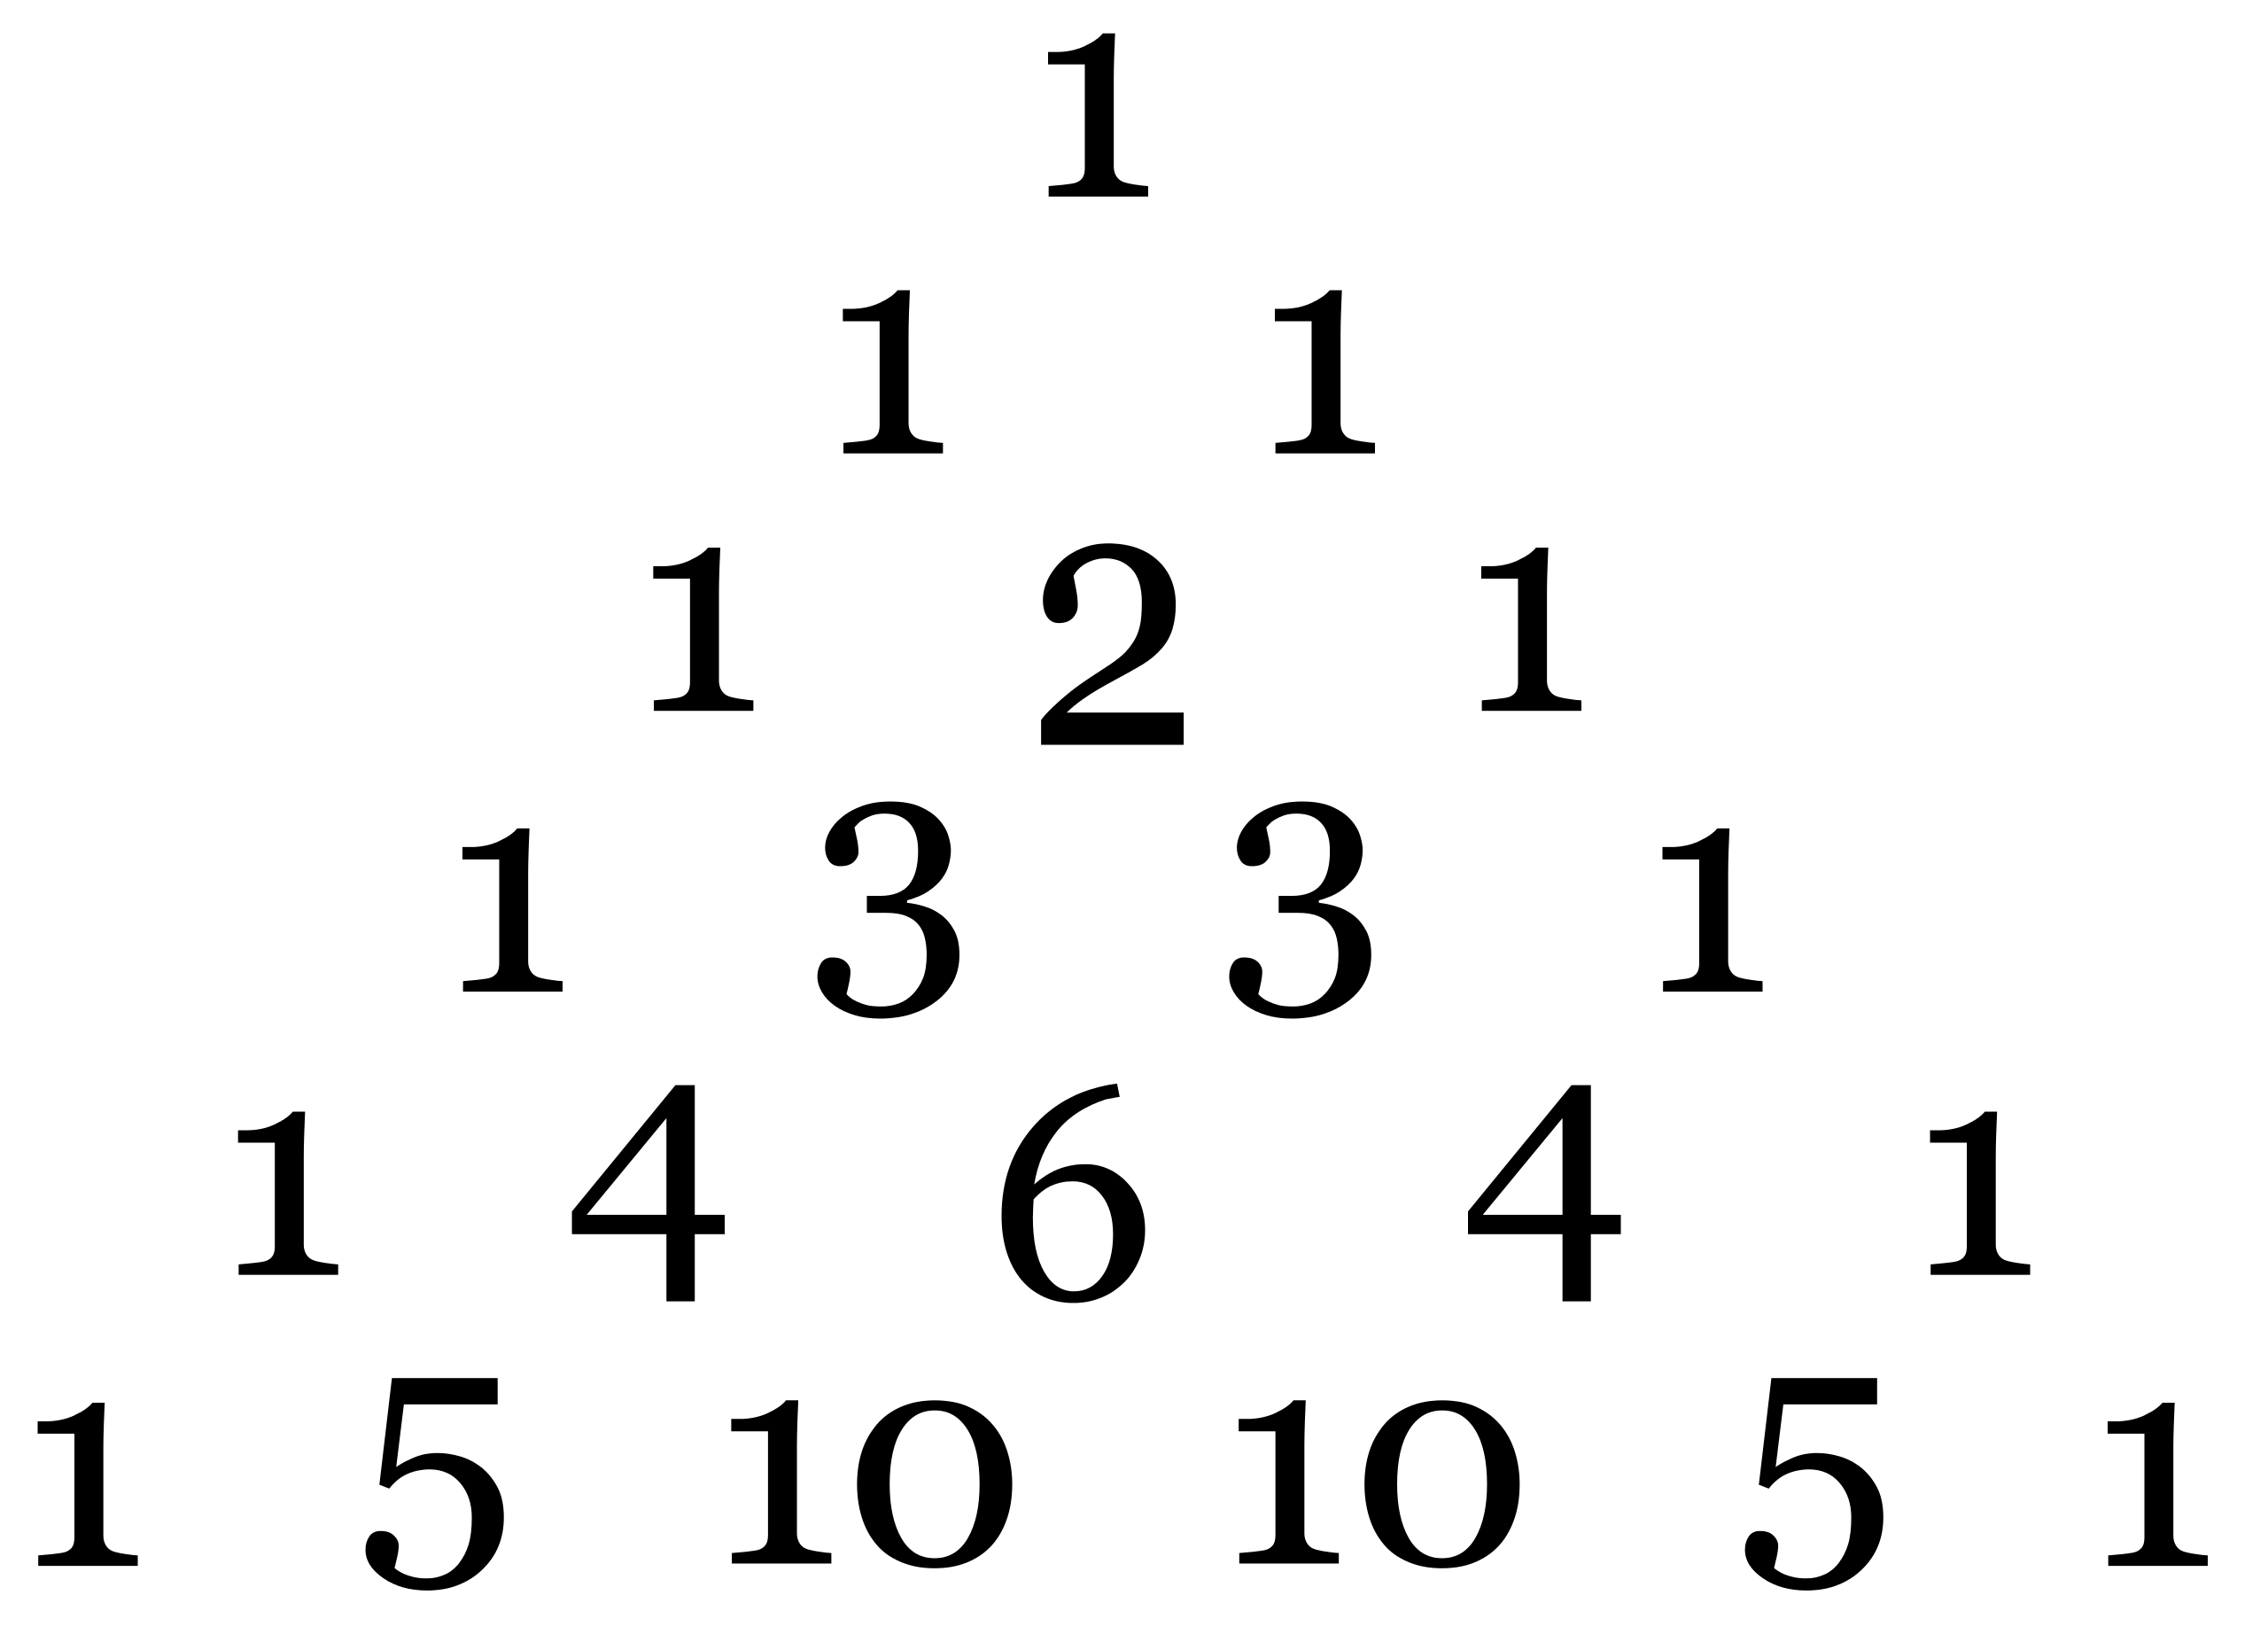
\includegraphics[width=0.4\linewidth]{src/images/pascals-triangle.png}
	\caption{杨辉三角形(又名帕斯卡三角形)}
	\label{fig:pascals-triangle}
\end{figure}

\subsection{应用}
熟练掌握组合数的性质和二项式展开的通项公式,可以解决大部分问题。对于另外一些问题,我们说不定还要深究二项式展开的根本思想。

\begin{example}
	已知$(\sqrt{x}-\frac{3}{x})^n$展开式只有第$5$项的二项式系数最大,求

	\begin{enumerate}
		\item $n$的值
		\item 展开式中$x^{-2}$的系数
		\item 所有有理项
	\end{enumerate}
\end{example}

\begin{proof}[解小题$1$]
	要第5项最大,根据组合数的性质得该数一定位于数列中央,故一共有9项,得$n=8$。
\end{proof}

\begin{proof}[解小题$2$]
	我们要先求出通项公式\[T_{r+1}=C_8^r(\sqrt{x})^{8-r}(-\frac{3}{x})^r=C_8^r(-3)^rx^{4-\frac{3}{2}r}\]

	使$x$的指数处等于$-2$,得\[4-\frac{3}{2}r=-2\Rightarrow r=4\]

	回代到通项公式得\[a=C_8^4(-3)^4=5670\qedhere\]
\end{proof}

\begin{example}
	求$(a-2b+3c)^{10}$展开式中$a^2b^3c^5$的系数.
\end{example}

\section[多项式问题]{用赋值法解决多项式问题}
对于一个多项式$(x+a)^n$,已知其展开式为\[k_0+k_1x+k_2x^2+\cdots+k_nx^n\]我们就可以依据展开式给$x$赋值直接或间接地求出一些系数的线性组合的值。

如果我们要求常数项的值,可令$x$为0;求各项系数之和,则令$x$为1。

\begin{example}
	已知$(3x-1)^8=a_0+a_1x+a_2x^2+\cdots+a_8x^8$,求

	\begin{enumerate}
		\item 求各项系数之和
		\item 求各二项式系数之和
		\item 求$a_0-a_1+a_2-\cdots+a_8$
		\item 求$a_0+a_2+\cdots+a_8$
		\item 求$a_1+a_3+\cdots+a_7$
		\item 求$\dfrac{a_1}{2}+\dfrac{a_2}{4}+\cdots+\dfrac{a_8}{2^8}$
	\end{enumerate}
\end{example}
